\documentclass{article}

\title{纯 Rust 中文排版引擎}
\subtitle{交付说明：从语法到 PDF 的一条可复现管线}
\author{soma-typeset}
\date{2026-11-20}

\begin{document}

\section{定位与边界}

一句话：一个用纯 Rust 写的中文优先排版引擎。Markdown、HTML、LaTeX（Word 在建）进来，按一份纯 YAML 模板，出去是同一套确定性的 PDF、HTML、SVG 与页面 JSON。

它不解决“把文字放到页面上”——浏览器做得够好。它解决三件浏览器做不好的事：

\begin{itemize}
\item 断行是\textbf{全局求解}。一段文字的所有断点一起优化，代价函数由每行的松紧、固定行数、标点挤压量、中英边界偏差与末行长短相加而成，每一项都能单独标定、单独解释。谁把哪一行换到了哪里，可以逐行打出账本。
\item 中文标点按规则处理，不靠空白。行首禁则、行尾禁则、标点对挤压、行末悬挂、行边裁剪，都是可关闭、可测量、可回归的规则，不是“看起来差不多”。
\item 同一份输入必须得到\textbf{同一份字节}。全部整数坐标、无浮点、字段顺序固定的 canonical JSON，native 与 wasm 逐字节同哈希。排版结果可以进版本库、可以做二进制比对。
\end{itemize}

明确不做的事：整书级跨页优化、竖排、双向文字、首字下沉、英文断词、脚注跨页拆分、图片绕排。这些不是“以后补”，而是模型边界；写进 \texttt{docs/debt.md} 的每一条都有触发条件。

\section{交付清单}

表格里的“阶段”是仓库里的真实里程碑，每个阶段的产物都带测试与门禁。

\begin{itemize}
\item \textbf{K1–K8 行内内核}：代价模型、行边裁剪、强制断行、降级阶梯、参数预设。已冻结。
\item \textbf{A1–A6 架构}：DocIR、模板与样式、盒子树、分页、三个前端、三个渲染器。已交付。
\item \textbf{E1–Q' 能力与质量}：表格、图片、注解、目录索引、书签、跨端哈希、效果评分。已交付。
\item \textbf{F1–F5 字体}：字体指纹、度量表、逐字选面、多字体混排。已交付。
\item \textbf{数学}：定界符、矩阵、斜体变量、编号与标签、拼接括弧。已交付。
\item \textbf{长文档}：目录、图目录、表目录、索引、PDF 书签、前置页页码。已交付。
\end{itemize}

规模：工作区 \textbf{18 个 crate}，\textbf{58 份 ADR}，\textbf{633 个测试}，全部通过 \texttt{cargo fmt}、\texttt{clippy -D warnings} 与 9 组门禁。

\section{一条管线}

管线只有一条，每一层只知道下一层的契约：

\begin{verbatim}
.tex / .md / .html
  -> frontend   语法到语义，产出 DocIR（soma.doc/2）
  -> template   样式解析，产出 Styled Doc（soma.template/9）
  -> layout     度量、断行、分页，产出 Result（soma.pages/10）
  -> render     PDF / HTML / SVG / JSON
\end{verbatim}

分层的硬纪律由脚本检查，不由自觉保证：\texttt{soma-core} 不允许依赖字体解析、Markdown 解析、序列化库或 wasm 绑定；\texttt{soma-doc} 不允许出现任何物理样式字段；模板不允许出现引擎参数。越界即门禁失败。

断行发生在两个尺度上：行内是 Knuth--Plass 动态规划，行间是垂直方向的 K-P 或贪心分页；脚注改变页面剩余高度，所以脚注与正文一起迭代求解，而不是先排正文再补脚注。

\section{排版能力}

\begin{itemize}
\item \textbf{断行}：全局 K-P、行边裁剪、标点悬挂、禁则、强制断行、应急与救援阶梯。
\item \textbf{标点}：标点对挤压、行末半宽字削边、行首行尾禁则、中英边界字距。
\item \textbf{分页}：行级垂直 K-P、孤行寡行惩罚、表格跨页续排、章节起始母版。
\item \textbf{结构}：标题、列表、引文、代码块、表格（跨行跨列、续排重复表头）、图片。
\item \textbf{长文档}：封面、目录（含图目录表目录）、索引、PDF 书签、前置页罗马页码。
\item \textbf{数学}：分式根式、大运算符、定界符、矩阵与 cases、斜体变量、编号与标签。
\item \textbf{字体}：TTF 与 CFF、按字族选面、逐字回退、子集化嵌入、度量表指纹。
\item \textbf{输出}：PDF（带标签结构）、HTML、SVG、canonical JSON。
\end{itemize}

几个值得单独说的点：

\begin{itemize}
\item 表格跨页按“行带”切分，切点只落在安全行边界；跨行单元格整体搬走而不是裁断；续页自动重复表头。
\item 目录与索引的页码来自第二遍排版，目录行本身也能换行，引导点跟随最后一行。
\item PDF 用动态 Huffman 压缩内容流，字体按实际用到的字形做子集，CFF 只保留闭包内的子程序。
\end{itemize}

\section{数学子集}

数学是一个可用的子集，不是 TeX 的替代品：分式、根式、大运算符、定界符伸缩、\texttt{matrix} 家族与 \texttt{cases}、\texttt{aligned} 按 \& 对齐、\texttt{array} 列格式、\texttt{substack} 堆叠、片语内的 \texttt{text} 与其中的公式、颜色、公式编号与自定义标签。

变量按数学习惯排斜体（面里有斜体区才启用，否则保持正体，不画方框），函数名与文字模式保持正体。宽括弧在字形会被拉平时改用线段拼：横杆、两个四分之一圆钩、一个尖，和 TeX 拼括弧是同一套零件。

\begin{equation}
\overbrace{a+b+\cdots+z}^{26}
\end{equation}

多行公式每行各自编号，标签不占用自动编号：

\begin{align}
\text{行宽} &= W - 2m \\
\text{压缩量} &= \frac{s}{S} \cdot D \notag \\
e &= mc^2 \tag{A}
\end{align}

\section{字体、度量与确定性}

\subsection{度量与选面}

排版只认宽度，不认字体。宽度从一张 \texttt{.smt} 度量表来：每一面记录字宽、升部、降部、行距与字形边距，由字体文件离线生成，带内容指纹。断行器拿到的只是整数。

\begin{itemize}
\item 同一次排版里可以同时有宋体正文、宋体粗体强调、黑体标题、等宽代码、数学面与楷体回退面；样式里的 \texttt{font-family} 决定用哪一族，缺面时静默回退而不是报错。
\item 一个字形在数学面上缺失时（例如公式里的汉字），度量与绘制都改走正文字面，两者用同一条规则，所以宽度和位置不会打架。
\item \texttt{soma.metrics/4} 的读取器兼容旧版本表；表变了，哈希就变，排版结果自然跟着变。
\end{itemize}

\subsection{可复现}

可复现不是“在同样环境里重跑一次”，而是三条硬约束：

\begin{itemize}
\item 所有几何量是 1/4096 em 的整数，除法的余数按边界顺序分配，没有浮点参与任何决策。
\item 结果写成字段顺序固定的 canonical JSON，\texttt{usize} 不进序列化，同一份输入在同一版本下逐字节相同。
\item 参数、模板、样式、引擎配置、度量表各有哈希，合成结果哈希；native 与 \texttt{wasm32-wasip1} 构建出同一串字节。
\end{itemize}

最后一条由门禁强制：同一份 fixture 分别用本机二进制与 wasm 模块跑，比较字节，不一致即失败。

\section{质量与验证}

验证不靠人眼抽查，靠四层：

\begin{itemize}
\item 暴力参考解：n 不超过 16 时枚举所有断点组合，与动态规划的最优代价逐条比对。
\item 硬不变量：K-P 的总代价不劣于贪心；非末行、无裁剪时行宽等于目标宽；禁则断点数恒为零。
\item 黄金样例与逐端哈希：同输入同字节，跨 native/wasm 一致，SVG 坐标与布局整数对得上。
\item 语料评测：9 篇中文文档、48 页、599 段、1213 行，统计强制压缩、应急行、孤行寡行、行间比例跳变与边界偏差误差。
\end{itemize}

\begin{table}
\caption{语料基线}
\begin{tabular}{lr}
\hline
指标 & 数值 \\
\hline
总行数 & 1213 \\
强制压缩行 & 0 \\
应急行 & 0 \\
孤行 / 寡行 & 0 / 0 \\
行间比例跳变 & 3 \\
边界偏差误差 p95 & 9‰ \\
\hline
\end{tabular}
\end{table}

读法：1213 行里没有一行被压到不自然的程度，也没有一行触发放宽容忍度，没有孤行寡行；行间松紧只反跳 3 次；代价模型估的边界偏差与真实分配量相比，95\% 的行在 9‰ 以内。

性能（单机 release，同一台机器）：纯中文 2000 字符段 p95 约 0.3 ms；中英混排 2000 字节约 20 ms、4000 字节约 80 ms，峰值内存约 4 MB。混排更慢是因为它真的在解 $O(n^2)$ 的动态规划，而不是走长度降级。

\section{实物}

三份样例都来自仓库里的源文件，一条脚本重渲：

\begin{table}
\caption{样例实测}
\begin{tabular}{llll}
\hline
文档 & 页数 & 体积 & 嵌入字体面 \\
\hline
宋体样张 & 13 & 1.19 MB & 6 \\
示例书 & 11 & 183 KB & 2 \\
案例集 & 49 & 507 KB & 2 \\
\hline
\end{tabular}
\end{table}

\begin{figure}
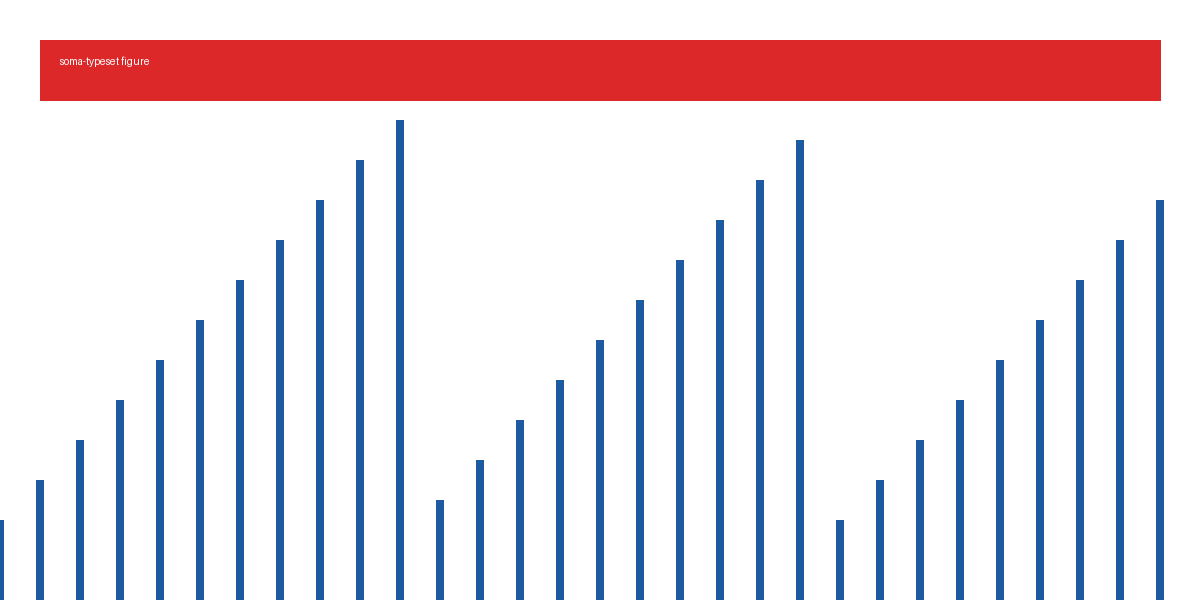
\includegraphics[width=0.9\linewidth]{fig/pipeline.png}
\caption{一张 PNG 位图：无损路径，像素由后端解码后压进 PDF}
\end{figure}

\begin{figure}
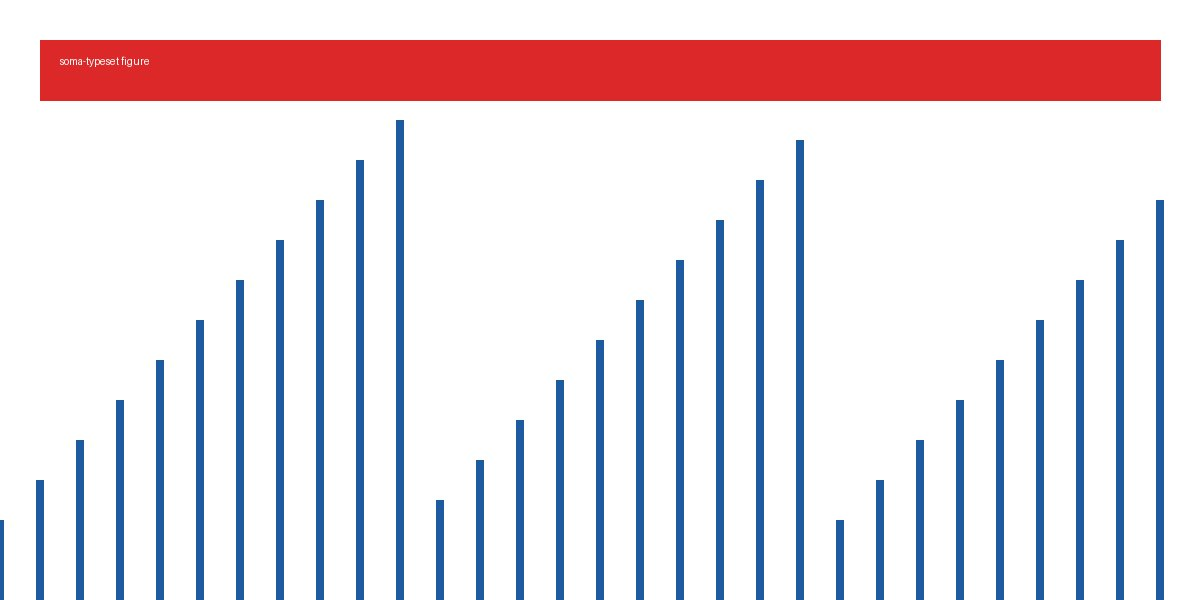
\includegraphics[width=0.8\linewidth]{fig/photo.jpg}
\caption{一张 JPEG 位图：原样直通，阅读器自己解码}
\end{figure}

三份 PDF 都带标签结构（标题、段落、表格行与单元格、公式），可以被屏读软件按结构走一遍；书签来自标题层级，页码与版心一致。

\begin{quote}
判断一个排版引擎是否成熟，不看它排得出一页漂亮的东西，而看它排糟的时候能不能说清糟在哪一行、哪个代价项、哪次迭代。
\end{quote}

\section{边界与下一步}

诚实的边界，按影响排序：

\begin{itemize}
\item 段落级优化，不做跨段、跨页的整书优化。相邻两页的灰度不参与同一个目标函数。
\item 数学是可用的子集：没有 \texttt{intertext}、没有 \texttt{alignat}，标签不排成独立的一列，拼出来的括弧比例固定而不是读字体的 MATH 表。
\item 英文不拆词，超长英文单词允许溢出，而不是硬断。
\item 索引按 Unicode 码位排序，没有中文拼音或笔画排序。
\item 脚注不跨页拆分，特高的脚注会把正文挤走而不是自己断开。
\end{itemize}

下一步优先级：Word 前端、图片混排、索引排序规则、以及把内容流压缩与字体子集再压一轮。

\subsection{复现命令}

\begin{verbatim}
cargo run -p soma-cli -- render \
  --input brief.tex --template song.yaml \
  --metrics song.smt --format pdf \
  --font      SourceHanSerifCN-Regular.otf \
  --font-bold SourceHanSerifCN-Bold.otf \
  --font-sans MiSans-Normal.ttf \
  --font-math NotoSansMath-Regular.ttf \
  --out brief.pdf
\end{verbatim}

门禁一行：\texttt{bash scripts/gates.sh}。它按顺序跑格式、静态检查、全量测试、wasm 交叉编译与哈希、示例渲染、依赖边界、架构检查与效果评分，任何一项失败都会停在那一步。

\end{document}
